\documentclass[]{article}
\usepackage[]{algorithm2e}
\usepackage{amsmath}
\usepackage{framed}
\usepackage{tabularx}
\usepackage[dutch]{babel}
\usepackage{graphicx}
\usepackage{epstopdf}

%opening
\title{Practicum NMB: Benaderende functies}
\author{Matthijs van Keirsblick en Harald Sch\"{a}fer}
\date{donderdag 14 mei 2015}

\newcommand{\opgave}[1]{\pagebreak\section*{Opgave #1}}


\begin{document}

\maketitle
\opgave{1}
\section*{Ellips}
Voor het berekenen van de coefficienten ellips lossen we het gegeven stelsel op naar b,c,d,e en f.
\\

 \begin{center}
 $
 \begin{bmatrix}
  2x_{1}y_{1} & y_{1}^2-x_{1}^2 & x_{1} & y_{1} & 1 \\
   2x_{1}y_{1} & y_{1}^2-x_{1}^2 & x_{1} & y_{1} & 1 \\
  \vdots  & \vdots  & \vdots & \vdots & \vdots \\
   2x_{1}y_{1} & y_{1}^2-x_{1}^2 & x_{1} & y_{1} & 1 \\
 \end{bmatrix}
 .
  \begin{bmatrix}
  b\\
  c\\
  d\\
  e\\
  f\\
  \end{bmatrix}
  =
   \begin{bmatrix}
    -x^2_1\\
   -x^2_2\\
    \vdots\\
   -x^2_N\\
    \end{bmatrix}
    $
     \end{center}

\noindent Hieruit kunnen we dan ook gemakkelijk a berekenen met de normalisatievoorwaarde $a = 1-c$. In figuur 1 zien we de resulterende ellips die een aantal willekeurige punten benadert.
\\
\begin{figure}[h]
\begin{center}
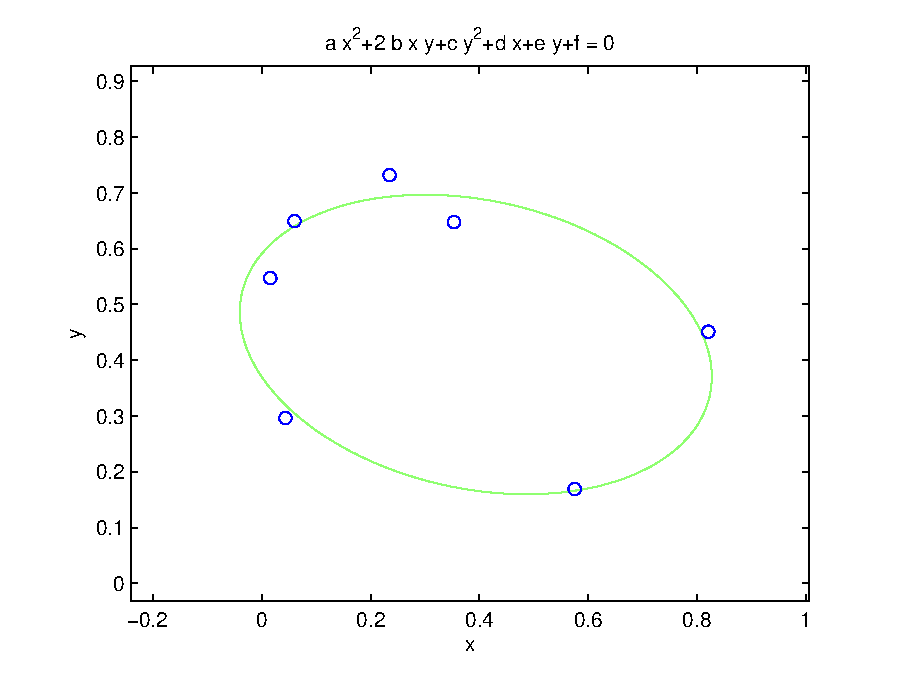
\includegraphics[width=1\textwidth]{ellips.eps}
\end{center}
\caption{Benaderende ellips voor een aantal willekeureige punten}
\end{figure}



\section*{Cirkel}
\noindent Voor het berekenen van de coefficienten van een benaderende cirkel beginnen we weer van de vergelijking:

 \begin{center}
 $ax^2 +2bxy + cy^2 + dx +  ey + f = 0$
 \end{center}
Daarin vullen we de normalisatievoorwaarde in en de voorwaarde van een cirkel, deze zijn:

 \begin{center}
 $ a = 1$	   \quad \quad \quad      	$b = 0$    \quad \quad \quad   	$a = c$
 \end{center}
 
 \noindent Dit geeft ons de vergelijking:
 
 \begin{center}
  $x^2 + y^2 + dx +  ey + f = 0$
  \end{center}
  
  \noindent Het stelsel om op te lossen wordt dan:
   
   \begin{center}
   $
   \begin{bmatrix}
    x_{1} & y_{1} & 1 \\
    x_{1} & y_{1} & 1 \\
   \vdots & \vdots & \vdots \\
    x_{1} & y_{1} & 1 \\
   \end{bmatrix}
   .
    \begin{bmatrix}
    d\\
    e\\
    f\\
    \end{bmatrix}
    =
     \begin{bmatrix}
      -y^2_1-x^2_1\\
      -y^2_2-x^2_2\\
      \vdots\\
      -y^2_N-x^2_N\\
      \end{bmatrix}
      $
       \end{center}
 
 \noindent In figuur 2 zien we de benaderende cirkel berekend met deze methode voor een aantal willekeurige punten.
 
 \begin{figure}[h]
 \begin{center}
 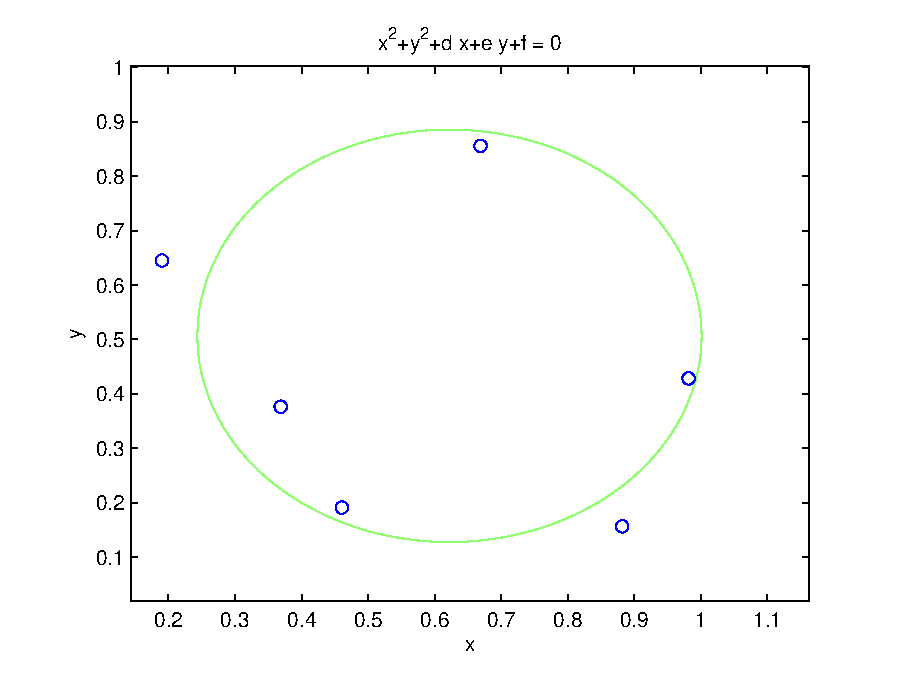
\includegraphics[width=1\textwidth]{cirkel.eps}
 \end{center}
 \caption{Benaderende cirkel voor een aantal willekeureige punten}
 \end{figure}
 
 \pagebreak
 \section*{Tekenkegelsnede}
 
 De vergelijking van de kegelsnede in het aangepast assenstelsel is 
\begin{center}
 $\lambda_1 \bar{x}^2 + \lambda_2 \bar{y}^2 + \bar{c} = 0$
\end{center} 
Om een ellips(of cirkel) te zijn moet $\lambda_1 > 0$, $\lambda_2 > 0$ en $\bar{c} \ge 0$. $\lambda_1$ en $\lambda_2$ zijn de eigenwaarden van de matrix:

\begin{center}
$		A
		=
     \begin{bmatrix}
      a & b \\
      b & c\\
      \end{bmatrix}
      $
      \end{center}
      
\noindent $\bar{c}$ vinden we uit de volgende vergelijkingen.


\begin{center}
      $		B
		=
     \begin{bmatrix}
      d \\
      f
      \end{bmatrix}
      $
      \quad \quad \quad
      $2T^tA = -B^t$
      \quad \quad \quad
      $\bar{c} = T^tAT + B^tT +f$
      \end{center}

\noindent We hebben nu alle nodige vergelijkingen om na te kijken of de coefficienten a,b,c,d,e en f voldoen aan de voorwaarden van een ellips(of cirkel). We hebben onze functie getest door de volgende testen uit te voeren.


\begin{itemize}
  \item tekenkegelsnede() uitgevoerd op de coefficienten berekend door ellips() toegepast op punten liggend op een willekeurige ellips, het resultaat was zoals verwacht 1
  \item tekenkegelsnede() uitgevoerd op de coefficienten berekend door cirkel() toegepast op punten liggend op een willekeurige cirkel, het resultaat was zoals verwacht 1
  \item tekenkegelsnede() uitgevoerd op de coefficienten berekend door ellips() toegepast op punten liggend op een rechte, het resultaat was zoals verwacht 0
\end{itemize}

\end{document}

